
\section*{Правила оформления библиографических источников}

Для добавления нового библиографического источника необходимо выполнить следующие шаги:
\begin{itemize}
	\item Убедиться, что нужный источник еще не присутствует в файле biblio.bib, который находится в репозитории с исходными текстами Стандарта OSTIS. В настоящее время все библиографические источники изначально описываются в этом файле.
	\item Добавить в файл biblio.bib описание библиографического источника в соответствии с форматом описания BibTex. Более подробно про формат можно почитать на сайте https://www.bibtex.com/g/bibtex-format/. Для помощи в оформлении можно использовать различные бесплатные средства, например, сервис https://www.doi2bib.org/ позволяет сгенерировать bib-описание на основе идентификатора DOI, кроме того, многие онлайн-библиотеки позволяют выгрузить описание нужного источника в формат BibTex.
	\item Каждому источнику в соответствии с форматом BibTex присваивается некоторое условное имя (цитатный ключ или просто ключ), по которому затем можно процитировать соответствующий источник. В рамках Стандарта OSTIS рекомендуется цитатные ключи источников в формате BibTex формировать путем транслитерации в латинский алфавит фамилии первого автора и добавления года издания источника, например:
	
	\begin{itemize}
		\item \textit{Trudeau1993}
		\item \textit{Golenkov2011}
	\end{itemize}
	
	Если при этом возникает неоднозначность, связанная с тем, что существует несколько работ того же автора в один год, то в конце ключа рекомендуется добавлять строчные латинские буквы a, b, c и так далее, например:
	
	\begin{itemize}
		\item \textit{Gribova2015a}
		\item \textit{Gribova2015b}
	\end{itemize}
	
	При формировании ключа для электронного источника или коллективной публикации, где невозможно выделить ключевого автора, рекомендуется формировать ключ из 1-2 английских слов или аббревиатур, позволяющих однозначно идентифицировать соответствующий источник. При использовании нескольких слов их можно соединять знаком нижнее подчеркивание, пробелы в ключах запрещены. При необходимости в конце ключа можно добавлять год издания. Например:
	
	\begin{itemize}
		\item \textit{IMS} (библиографическая ссылка на сайт Метасистемы OSTIS)
		\item \textit{CYPHER} (библиографическая ссылка на сайт с описанием языка Cypher)
		\item \textit{AIDictionary1992} (библиографическая ссылка на Словарь по искусственному интеллекту 1992 года издания)
	\end{itemize}

Для добавленного источника необходимо описать его идентификатор, который далее будет использоваться в рамках текста Стандарта. Это делается при помощи BibTex поля shorthand, например (см. \textit{Правила идентификации библиографических источников}):

\begin{verbatim}
shorthand = {Trudeau.R.J.IntroGT-1993кн}
shorthand = {Duchi.J..AdaptiveSubgradMethods-2011ст}
shorthand = {Грибова.В.В..БазоваяТРИСОП-2015ст}
\end{verbatim}

Далее этот идентификатор может использоваться как в формальном тексте, также как и идентификатор любой другой сущности, так и в рамках естественно-языкового текста. Для автоматической вставки идентификатора библиографического источника в формальный либо естественно-языковой текст используется команда \begin{verbatim}\scncite{<цитатный ключ>}\end{verbatim}

Пример исходного кода:

\begin{verbatim}
\scnheader{конвергенция\scnsupergroupsign}
\scnidtf{уровень конвергенции (близости)\scnsupergroupsign}
\scnsuperset{конвергенция кибернетических систем\scnsupergroupsign}
\begin{scnreltolist}{ключевой знак}
	\scnitem{\scncite{Yankovskaya2017}}
	\scnitem{\scncite{Palagin2013}}
	\scnitem{\scncite{Yankovskaya2010}}
	\scnitem{\scncite{Kovalchuk2011}}
\end{scnreltolist}		
\end{verbatim}

Результат компиляции:

\begin{SCn}
\scnheader{конвергенция\scnsupergroupsign}
\scnidtf{уровень конвергенции (близости)\scnsupergroupsign}
\scnsuperset{конвергенция кибернетических систем\scnsupergroupsign}
\begin{scnreltolist}{ключевой знак}
	\scnitem{\scncite{Yankovskaya2017}}
	\scnitem{\scncite{Palagin2013}}
	\scnitem{\scncite{Yankovskaya2010}}
	\scnitem{\scncite{Kovalchuk2011}}
\end{scnreltolist}
\end{SCn}

\item Для каждого источника крайне желательно добавить его краткую аннотацию. Это делается при помощи BibTex поля annotation, например:

\begin{verbatim}
annotation = {В этой книге представлены исследования по внедрению концептуальных основ, стратегий, методов, методологий, информационных платформ и моделей для разработки современных систем, основанных на знаниях}
\end{verbatim}

В рамках аннотации допускается использование средств форматирования естественно-языковых текстов, принятых в рамках Стандарта OSTIS, например, выделение курсивом или полужирным курсивом.

Для вставки аннотации в формальный scn-текст используется команда 

\begin{verbatim}
\scnciteannotation{<цитатный ключ>}
\end{verbatim}

Пример исходного кода:

\begin{verbatim}
\scnheader{\scncite{McBride2021}}
\scnciteannotation{McBride2021}
\end{verbatim}

Результат компиляции:

\scnheader{\scncite{McBride2021}}
\scnciteannotation{McBride2021}

\end{itemize}

\section*{Правила идентификации библиографических источников}

Идентификаторы статей, книг и других печатных работа строятся следующим образом:

\begin{itemize}
	\item Пишется фамилия первого автора на том языке, на котором опубликована данная работа. Затем через точку ставятся инициал(-ы) первого автора
	\item Если работа опубликована с участием только одного автора, то ставится одна точка, если нескольких - две точки
	\item Пишется первое слово из названия работы на том языке, на котором опубликована данная работа. Допускается сокращение, если слово очень длинное.
	\item Перечисляются Заглавные первые буквы всех остальных слов названия работы за исключением служебных слов, таких как предлоги, частицы, артикли и т.п.
	\item Ставится дефис
	\item Указывается год издания работы
	\item Указывается 2-3 буквенный код, обозначающий тип работы, например:
	\begin{itemize}
		\item \textit{кн} или \textit{bk} -- книга
		\item \textit{ст} или \textit{art} -- статья
	\end{itemize}
	
	Например:
	
	\textit{Мартынов.В.В.СемиологОИ-1974кн}

	Полное библиографическое описание:
	Мартынов В. В., Семиологические основы информатики, Минск, 1974
	
	\textit{Golenkov.V.V..MethodsTECCS-2019art}
	
	Полное библиографическое описание:
	Methods and tools for ensuring compatibility of computer systems / V. Golenkov [et al.] // Открытые семантические технологии проектирования интеллектуальных систем = Open Semantic Technologies for Intelligent Systems (OSTIS-2019) : материалы международной научно-технической конференции, Минск, 21 - 23 февраля 2019 г. / Белорусский государственный университет информатики и радиоэлектроники; редкол.: В. В. Голенков (гл. ред.) [и др.]. - Минск, 2019. - С. 25 - 52.
	
	\item Идентификаторы электронных и прочих ресурсов формируются аналогичным образом, с учетом того, что опускается год издания и фамилии авторов, а также ставится буквенный код \textit{эл} для обозначения электронного ресурса:
	
	\textit{МетасистIMS-эл} 
	\textit{Cypher-2017эл} 
	
\end{itemize}

\section*{Примеры библиографии в тексте}

Работа \scncite{Golenkov2018} посвящена вопросам обучения и обучаемости в интеллектуальных системах.

Работа \scncite{Wooldridge2009} описывает основные принципы многоагентных систем.

\section*{Примеры рисунков}

Рисунок \textit{\nameref{fig:example}} показывает, как надо оформлять рисунки. Размер рисунка можно задавать при помощи параметра scale.

\begin{figure}[H]
	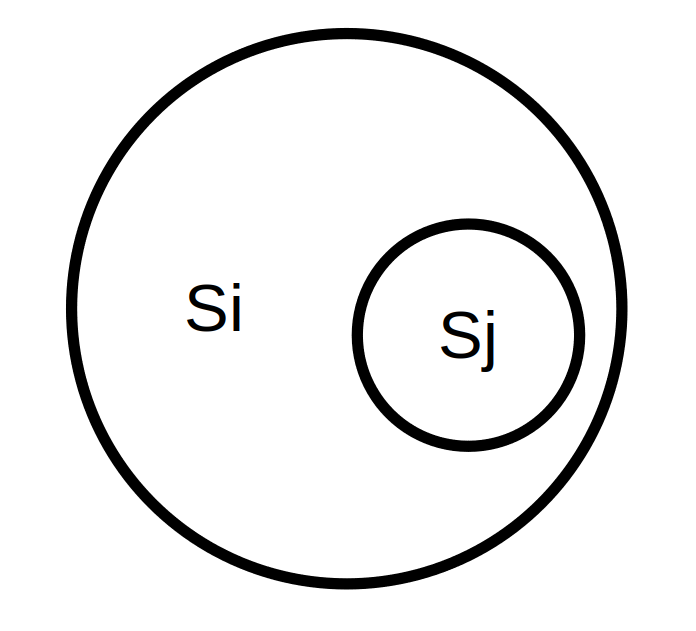
\includegraphics[scale=0.5]{images/fig_example.png}
	\caption{Пример обычного рисунка}
	\label{fig:example}
\end{figure}

Рисунок \textit{\nameref{fig:example_scg}} показывает, как надо оформлять рисунки в SCg-коде. Параметр scale должен быть выставлен равным 0.8, для того чтобы все рисунки в SCg-коде имели одинаковый масштаб и размер идентификаторов примерно соответствовал размеру шрифта основного текста.  

\begin{figure}[H]
	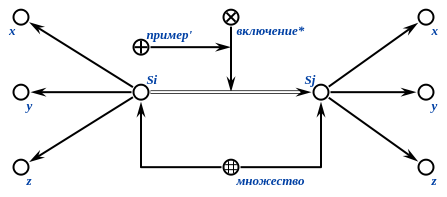
\includegraphics[scale=0.8]{images/fig_example_scg.png}
	\caption{Пример рисунка в SCg-коде}
	\label{fig:example_scg}
\end{figure}
